\documentclass[../Head/Main.tex]{subfiles}
\begin{document}
\begin{figure}[H]
  \begin{subfigure}[b]{0.49\textwidth}
    \centering
    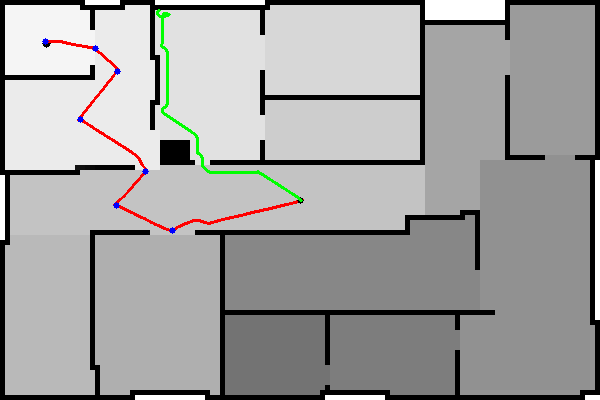
\includegraphics[width=0.9\textwidth]{Modelbased_vs_Sensorbased/brushfireAndBugTest1}
    \caption{Illustration of the run from the origin to room 1}
    \label{fig:Test1}
  \end{subfigure}
  \hfill
  \begin{subfigure}[b]{0.49\textwidth}
    \centering
    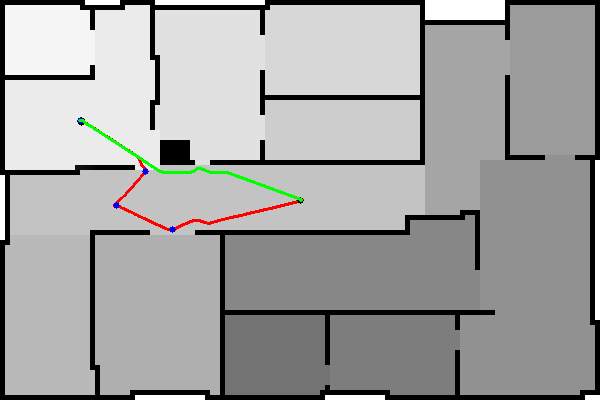
\includegraphics[width=0.9\textwidth]{Modelbased_vs_Sensorbased/brushfireAndBugTest2}
    \caption{Illustration of the run from the origin to room 2}
    \label{fig:Test2}
  \end{subfigure}
  \hfill
  \begin{subfigure}[b]{0.49\textwidth}
    \centering
    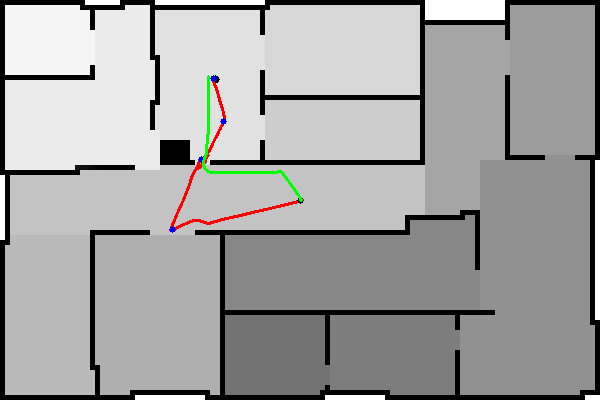
\includegraphics[width=0.9\textwidth]{Modelbased_vs_Sensorbased/brushfireAndBugTest3}
    \caption{Illustration of the run from the origin to room 3}
    \label{fig:Test3}
  \end{subfigure}
  \hfill
  \begin{subfigure}[b]{0.49\textwidth}
    \centering
    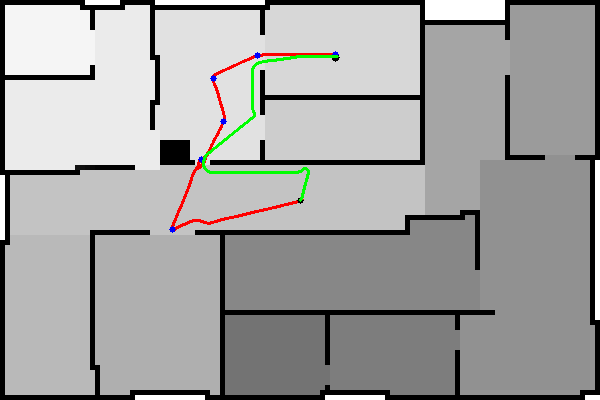
\includegraphics[width=0.9\textwidth]{Modelbased_vs_Sensorbased/brushfireAndBugTest4}
    \caption{Illustration of the run from the origin to room 4}
    \label{fig:Test4}
  \end{subfigure}
  \hfill
  \begin{subfigure}[b]{0.49\textwidth}
    \centering
    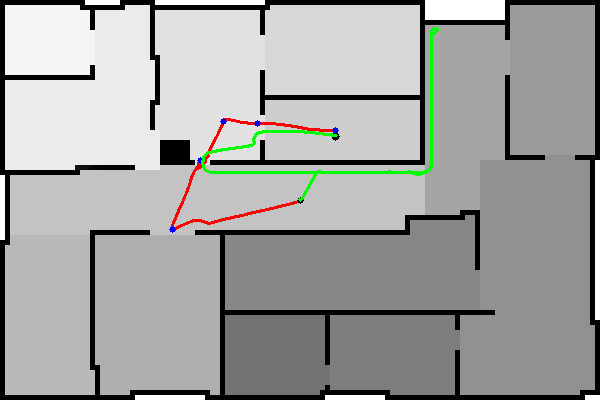
\includegraphics[width=0.9\textwidth]{Modelbased_vs_Sensorbased/brushfireAndBugTest5}
    \caption{Illustration of the run from the origin to room 5}
    \label{fig:Test5}
  \end{subfigure}
  \hfill
  \begin{subfigure}[b]{0.49\textwidth}
    \centering
    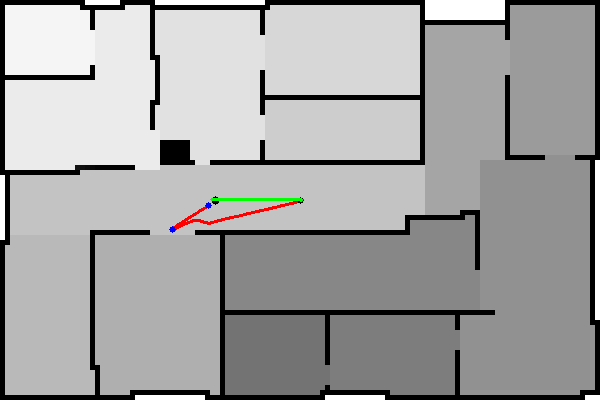
\includegraphics[width=0.9\textwidth]{Modelbased_vs_Sensorbased/brushfireAndBugTest6}
    \caption{Illustration of the run from the origin to room 6}
    \label{fig:Test6}
  \end{subfigure}
  \hfill
  \begin{subfigure}[b]{0.49\textwidth}
    \centering
    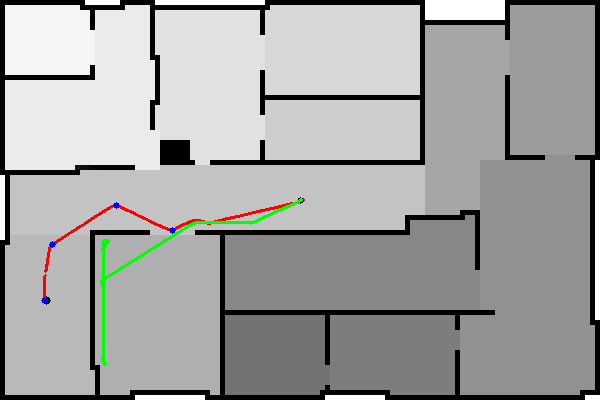
\includegraphics[width=0.9\textwidth]{Modelbased_vs_Sensorbased/brushfireAndBugTest7}
    \caption{Illustration of the run from the origin to room 7}
    \label{fig:Test7}
  \end{subfigure}
  \begin{subfigure}[b]{0.49\textwidth}
    \centering
    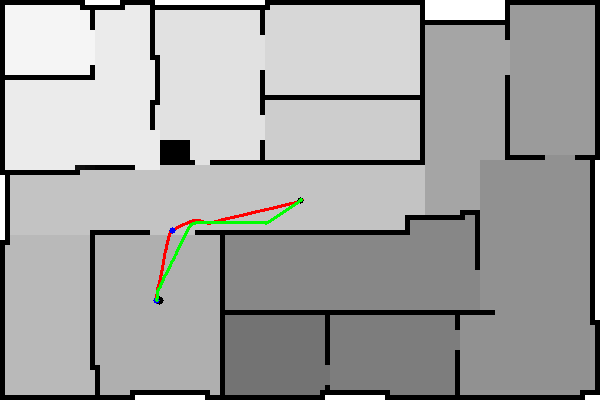
\includegraphics[width=0.9\textwidth]{Modelbased_vs_Sensorbased/brushfireAndBugTest8}
    \caption{Illustration of the run from the origin to room 8}
    \label{fig:Test8}
  \end{subfigure}
  \caption{Illustration of the run from the origin to room 1-8 for both the model based (red line) and the sensor based (green line)}
\end{figure}
\begin{figure}[H]
  \begin{subfigure}[b]{0.49\textwidth}
    \centering
    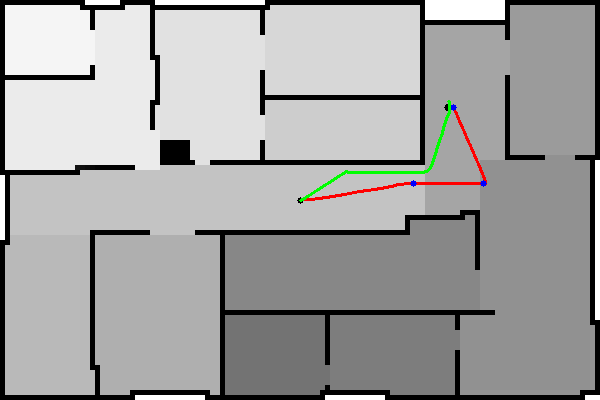
\includegraphics[width=0.9\textwidth]{Modelbased_vs_Sensorbased/brushfireAndBugTest9}
    \caption{Illustration of the run from the origin to room 9}
    \label{fig:Test9}
  \end{subfigure}
  \hfill
  \begin{subfigure}[b]{0.49\textwidth}
    \centering
    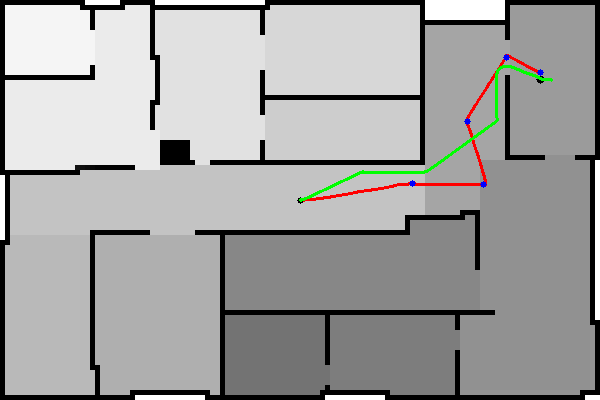
\includegraphics[width=0.9\textwidth]{Modelbased_vs_Sensorbased/brushfireAndBugTest10}
    \caption{Illustration of the run from the origin to room 10}
    \label{fig:Test10}
  \end{subfigure}
  \hfill
  \begin{subfigure}[b]{0.49\textwidth}
    \centering
    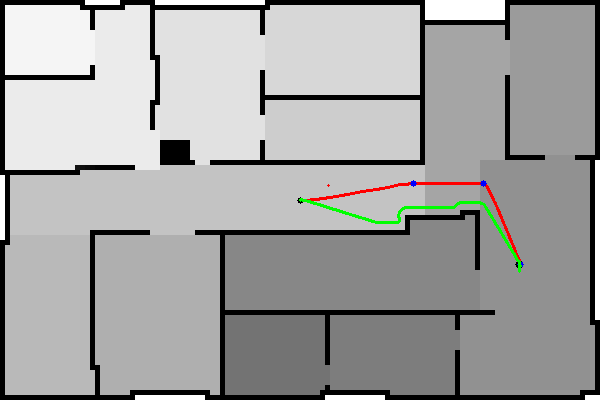
\includegraphics[width=0.9\textwidth]{Modelbased_vs_Sensorbased/brushfireAndBugTest11}
    \caption{Illustration of the run from the origin to room 11}
    \label{fig:Test11}
  \end{subfigure}
  \hfill
  \begin{subfigure}[b]{0.49\textwidth}
    \centering
    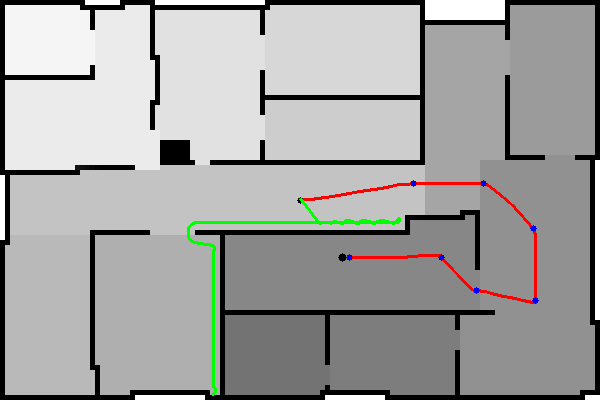
\includegraphics[width=0.9\textwidth]{Modelbased_vs_Sensorbased/brushfireAndBugTest12}
    \caption{Illustration of the run from the origin to room 12}
    \label{fig:Test12}
  \end{subfigure}
  \begin{subfigure}[b]{0.49\textwidth}
    \centering
    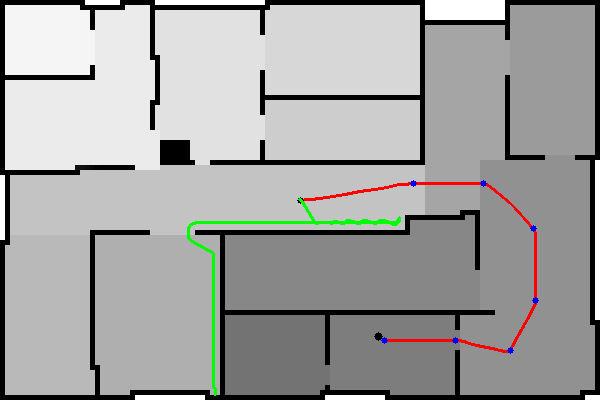
\includegraphics[width=0.9\textwidth]{Modelbased_vs_Sensorbased/brushfireAndBugTest13}
    \caption{Illustration of the run from the origin to room 13}
    \label{fig:Test13}
  \end{subfigure}
  \hfill
  \begin{subfigure}[b]{0.49\textwidth}
    \centering
    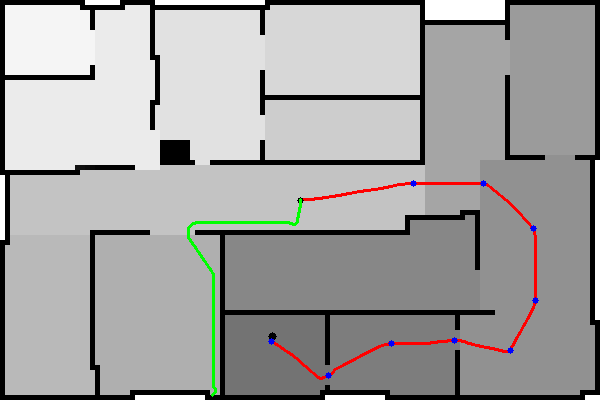
\includegraphics[width=0.9\textwidth]{Modelbased_vs_Sensorbased/brushfireAndBugTest14}
    \caption{Illustration of the run from the origin to room 14}
    \label{fig:Test14}
  \end{subfigure}
  \caption{Illustration of the run from the origin to room 9-14 for both the model based (red line) and the sensor based (green line)}
\end{figure}
\end{document}